
\section{Introduction}

W skład oprogramowania  \SoftwareName wchodzi moduł gry wykorzystujący silnik gry Unity oraz biblioteka wykonana w środowisku Matlab/Octave. Moduł gry może być sterowany za pomocą komend w których dane są zapisane formacie XML-a (fig.~\ref{Fig:architecture}). Odpowiada za wizualizację planszy gry oraz sterowanie jej przebiegiem. Domyślnie gra jest tak skonfigurowana, żeby nasłuchiwała na porcie 55001. Wpisany domyślnie adres (127.0.0.1) umożliwia łączenie się z grą tylko z komputera na którym jest ona zainstalowana (można to jednak zmienić).

 Biblioteka ma za zadanie ułatwić tworzyć oprogramowanie w Matlab-ie/Octave przeznaczone do testowania metod wspomagania decyzji.  Zawiera metody przygotowujące i formatujące komendy, które mają być przesyłane do gry. Umożliwia także dekodowanie otrzymanych od gry odpowiedzi. Dodatkową możliwością biblioteki jet konwersja tablic do formatu środowiska tabular Latex'a oraz formatu umożliwiającego odczytanie ich przez  moduł tworzenia wykresów pakietu tikz.

\begin{figure}
\begin{tikzpicture}
\node[rectangle,draw,minimum width = 3.5cm,minimum height = 1.5cm,label=above:{Player}] (r) at (-2.5,4.5) {Matlab/Octave};
\node[anchor=center,inner sep=0,label=above:{Game}] (game) at (4,4.5) {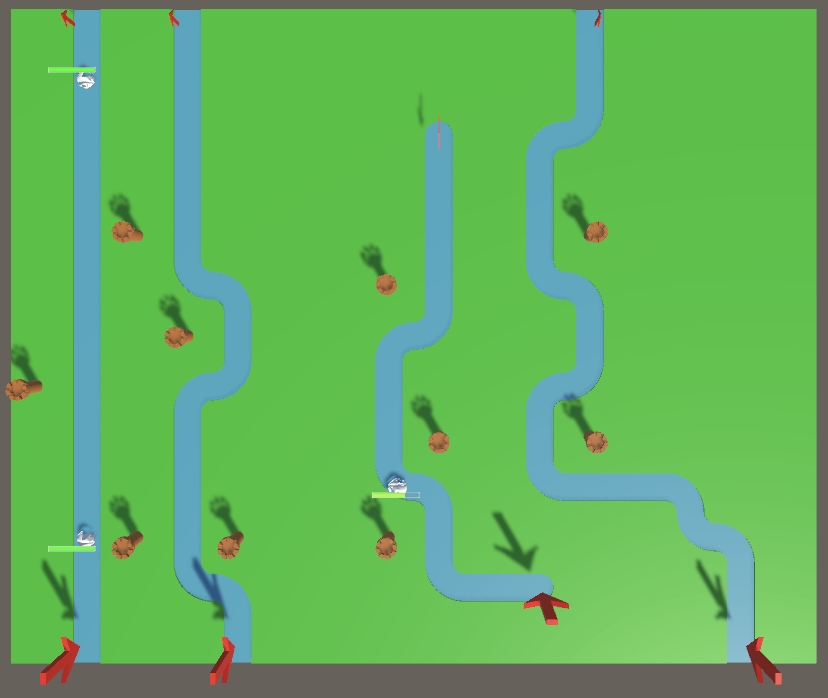
\includegraphics[width=3cm]{images/game.png}} ;
\node[anchor=center,inner sep=0, label=below:{Reports}] (tabaular) at (-2.5,1) {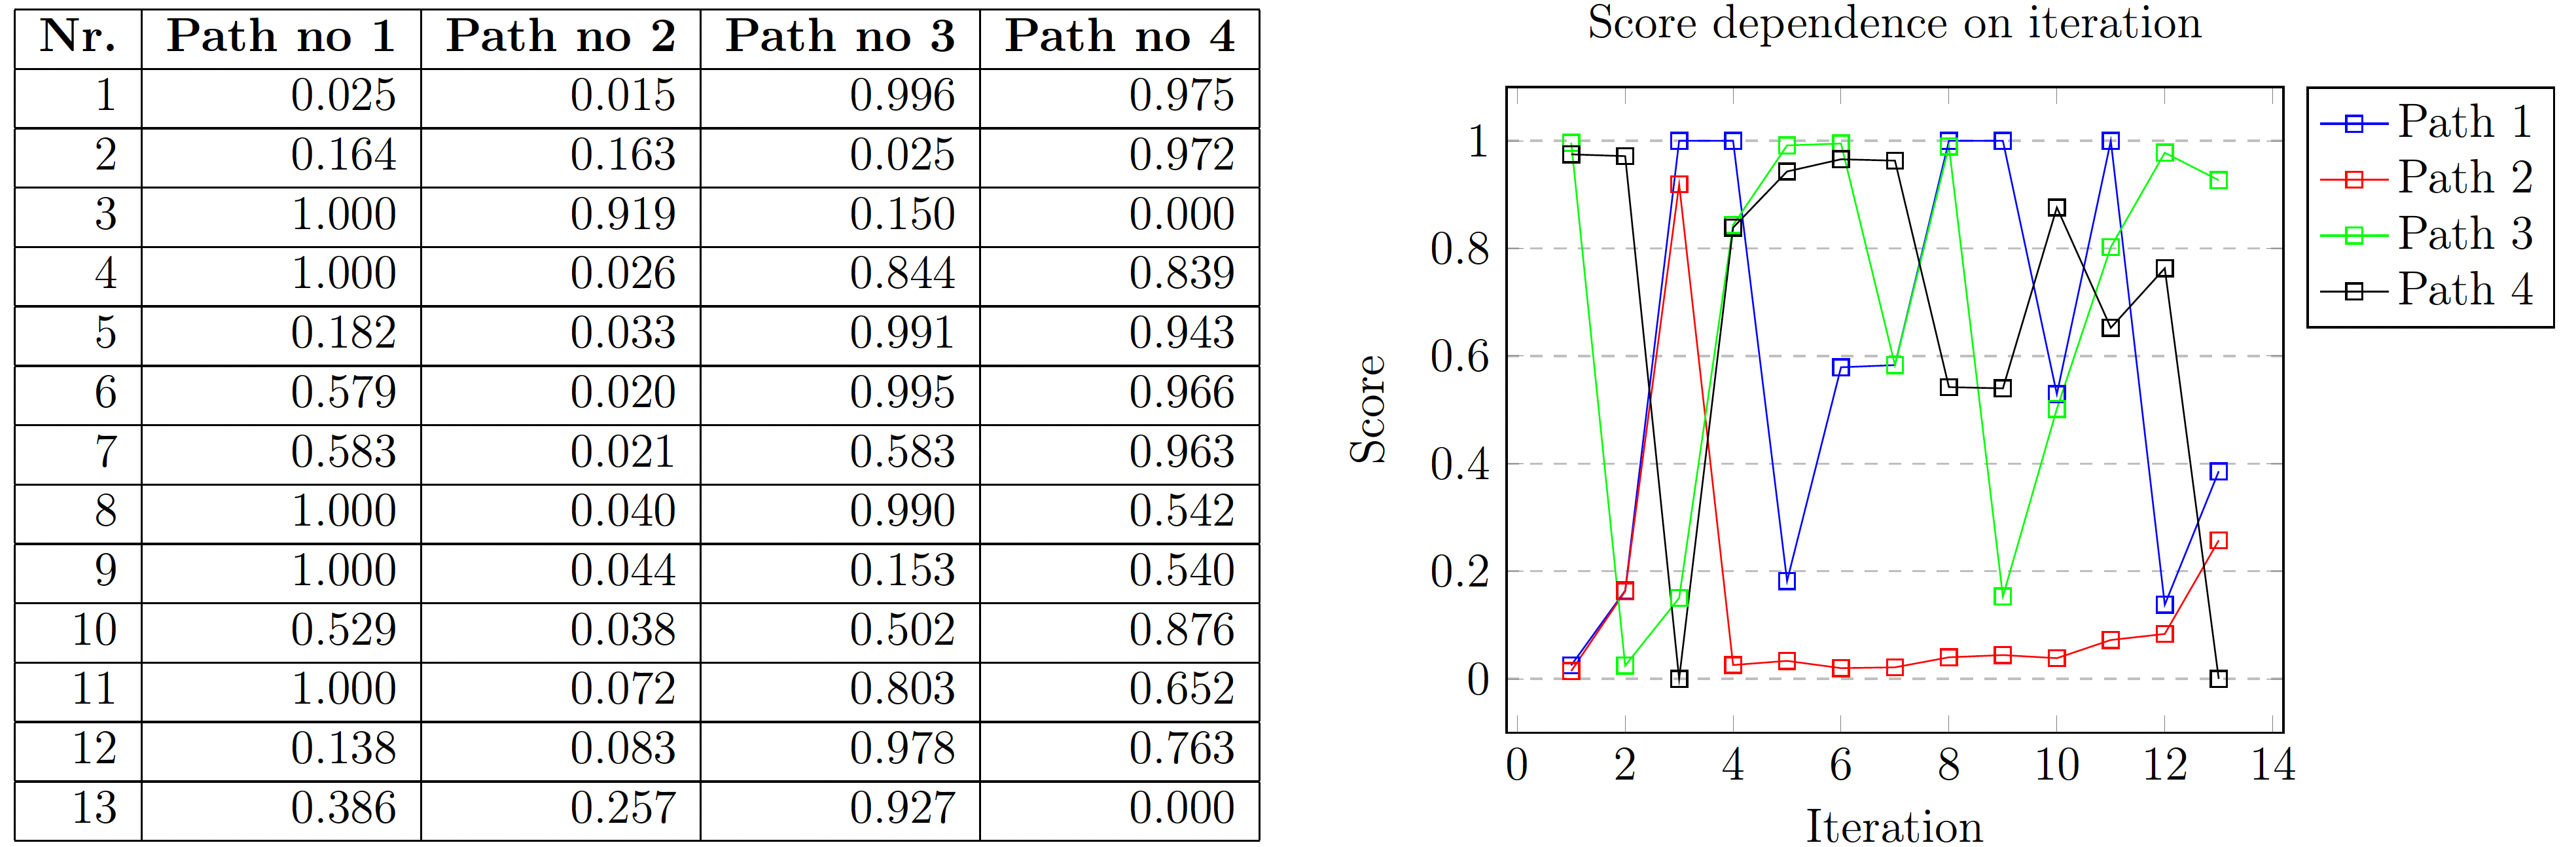
\includegraphics[height=2.5cm]{images/latexReports.png}};
\draw[oneArrowinverseStyle] (r.east) + (0,-0.1) -- ++(3.3,-0.1) node[midway,below]{Answer};
\draw[oneArrowStyle] (r.east) + (0,0.1) -- ++(3.3,0.1) node[midway,above]{Command};
\draw[oneArrowStyle] (r) -- (tabaular);

\end{tikzpicture}

\caption{Architektura systemu}
\label{Fig:architecture}
\end{figure}